
\section{Background}
\label{sec:optimizer:background}

Factor graphs
are a pairwise formalism for expressing arbitrarily complex
relationships between random variables~\cite{koller2009probabilistic}.
A factor graph $\mathcal{F} = \langle \textbf{x}, \psi \rangle$, contains a set of random
variables $ \textbf{x} = {\{x_i \}}^n_1$ and
factors ${\textbf{\boldmath$\psi$\unboldmath}} = { \{\psi_i\} }^m_1 $.
Random variables are connected to each other through factors.
Factors represent a mapping of the relationship to a real valued number.

The probability of a setting $\mathbf{\omega}$ among the set of all possible
settings $\Omega$ occurring in the factor graph is given by a probability measure:
\begin{align*}
\pi(\mathbf{\omega}) = \frac{1}{Z} \sum_{v \in \omega} \prod_{i=1}^{m} \psi_i(v^i) &,&  Z = \sum_{\omega \in \Omega} \sum_{v \in \omega}  \prod_{i=1}^{m} \psi_i(v^i) 
\end{align*}
where $v^i$ is the set of random variables that neighbor the factor
$\psi_{i}(\cdot)$ and $Z$ is the normalizing constant.


%Markov Chain Monte Carlo Metropolis Hastings is a techniques for performing
Exact inference over complex factors graphs is computationally expensive
because it involves computing the normalizing constant.
Therefore, it is popular for researchers to use Markov Chain Monte Carlo (MCMC) 
approximation techniques to estimate the probability of settings.
In particular, for large and dense factor graphs MCMC Metropolis Hastings (MH) has
been shown to be a scalable and effusive technique for 
inference calculation~\cite{singh2011large}.

Cross-Document entity resolution, resolving entities across document borders,
is usually several orders of magnitude smaller when compared to within document entity resolution.
In large text corpora, the sizes of entities follows the power law~\cite{singh12:wiki-links}.
For example, Figure~\ref{fig:entity-distribution} is a generated data set containing
40 million mentions and 3 million entities over 11 million web pages.
As documents and mentions are incrementally streamed through,
the scale problem must becomes a critical issue.

The mentions on disk can be represented as a large array of identifiers.
Entities are a collection of mentions and can be represented as such.
In the worst case there is an equal number of entities and mentions.
This means each mention is its own individual entity.
In the other extreme, all the mentions may be a part of the same entity.
For streaming entity resolution, mentions within documents (mention chains)
must be matched to the existing set of entities~\cite{rao2010streaming}.
In this paper, we assume the entity set is initialized by grouping the most
similar mentions; new mentions are assigned to the closed match.

Comparisons of the mentions in clusters is a factor of the number of pairwise links between mentions.
The pairwise factors include weighted functions such as approximate string matches, token overlap, ngram matches.
Additionally, cluster wide features are also computed and weighted.
Such features include functions to check whether all mentions in a cluster share the same token.
For clusters larger than 1000 mentions calculating scores of the model becomes extremely expensive.
Performing sophisticated techniques over smaller clusters also adds extra over head.
In this paper, we examine the trade-off of selecting techniques to
accelerate the feature computation process.


\begin{figure}
\centering
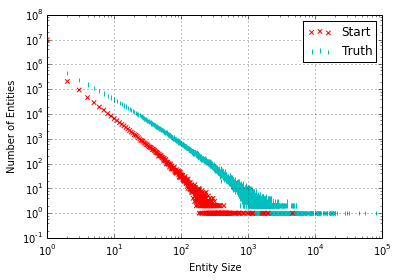
\includegraphics[width=\columnwidth]{media/start-vs-nd.png}
\caption{A distribution of entity sizes from the wiki-links corpus~\cite{singh12:wiki-links} with an initial start and the truth.}
\label{fig:entity-distribution}
\end{figure}



\section{Related Work}
\label{sec:optimizer:relatedwork}

In this paper, we focus on the creation of optimizers for sampling based ER over factor graphs.
We observe two seminal methods for increasing sampling speed.
First, is a method for approximating the score of factor counts and second is a compression method.
To this end, we look at three works that state-of-art techniques, respectively, for
 (1) early stopping methods,
 (2) entity resolution compression,
 (3) streaming entity resolution.
We use these works as a backdrop to development of the optimizer.

Singh et al.\ describe a method of approximating the factor computation during MCMC
inference over factor graphs~\cite{singh2011large}.
In this work, they note that sampling is usually inexpensive except in the case
of many variable, or if scoring a sample is low. To this end they introduce Monte
Carlo MCMC, this is a method of performing uniform and confident-based sampling
over the computation of factors to avoid the full computation of features.
This work shows significant speed up in a large-scale experiments.

% Slides: http://people.cs.umass.edu/~sameer/files/largescale-acl11-ppt.pdf
% Slides: http://people.cs.umass.edu/~sameer/files/mcmcmc-emnlp12-ppt.pdf

Wick et al.\ perform hierarchal compression of entities during
entity resolution~\cite{wick2013discriminative}.
This work defines a recursive data structure that allows succinct representations
of millions of mentions. 
The hierarchical structure adds some book keeping to the sampling process but because
large entity clusters are compress there are less comparison for each sampling iteration. 
This works displays orders of magnitude speedup
when compared to a pairwise method.

Rao et al.\ create a system for streaming entity resolution~\cite{rao2010streaming}.
The use the doubling algorithm~\cite{charikar1997incremental} to grow sets of clusters
and a clever disk arrangement strategy~\cite{omiecinski1984global} to retrieve
growing entities on demand.
However, this paper outlines no long-term strategy for managing growing entities.
The same pain points we identified with streaming entity resolution exist in this work.

%As we see, in Section~\ref{sec:microbenchmark} the entity sizes have a
%large effect on the factor computation size.


